\documentclass[10pt,a4paper]{article}
\usepackage{verbatim}
\usepackage{subcaption}
\usepackage{karnaugh-map}
\usepackage[utf8]{inputenc}
\usepackage[italian]{babel}
\usepackage{amsmath}
\usepackage{amsfonts}
\usepackage{amssymb}
\usepackage{graphicx}
\usepackage[left=2cm,right=2cm,top=2cm,bottom=2cm]{geometry}
\newcommand{\rem}[1]{[\emph{#1}]}
\newcommand{\exn}{\phantom{xxx}}
\renewcommand{\thesubsection}{\thesection.\alph{subsection}}  %% use 1.a numbering

\author{Gruppo EB.24 \\Giovanni Sucameli, Davide Incalza, Francesco Sacco}
\title{Ottica 2 B - Interferometro di Michelson}
\date{Aprile 2019}

\begin{document}
\maketitle
\section*{Scopo dell'esperienza}
	asd
\section*{Calcolo del motiplicatore}
	Come accennato nei cenni teorici lo spostamento $2\Delta x=n\lambda$, inoltre $\Delta x= k\Delta c$, dove $k$ è la costante moltiplicativa della leva e $c$ è la posizione del calibro.\newline
	\begin{equation}
		2k\Delta c=n\lambda
	\end{equation}
	per riuscire a contare $n$ (il numero di lunchezze d'onda passate) abbiamo fatto un video al rallentatore col telefono della figura d'interferenza, a questo punto abbiamo calcolato il centro di luce $C$ del dell'immagine d'interferenza e graficato la posizione y dell'immagine in funzione del numero di fotogrammi (immagine \ref{fig:cmy}).
	\begin{center}
		\begin{minipage}{.4\linewidth}
			\centering
			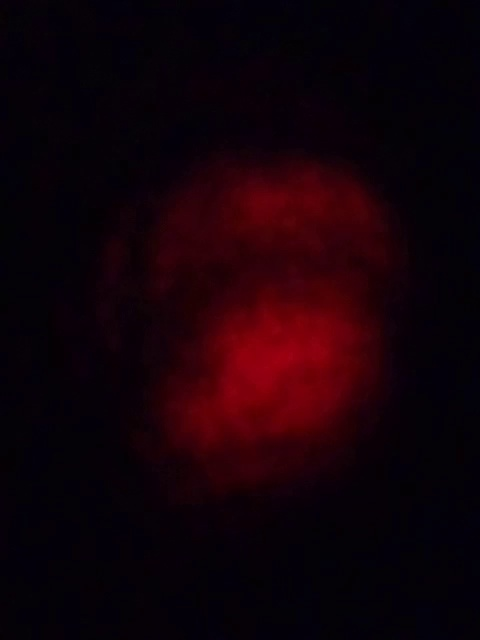
\includegraphics[width=0.43\linewidth]{dati/fotogrammi/500.jpg}
		\end{minipage}
		\rightarrow
		\begin{minipage}{.4\linewidth}
			\centering
			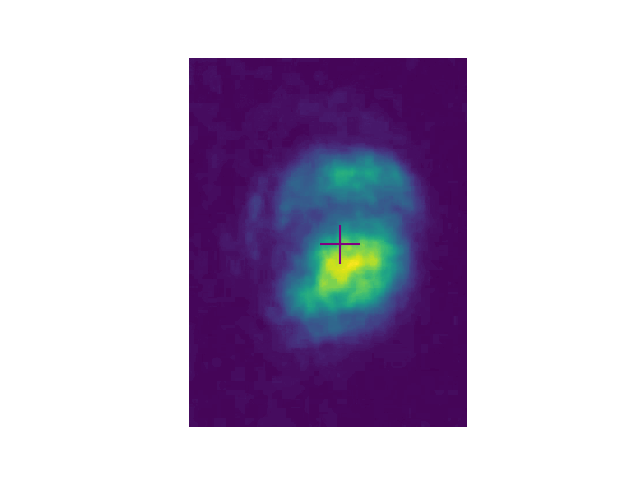
\includegraphics[width=\linewidth]{immagini/video/0500.png}
		\end{minipage}\\
	\caption{asd}
	\end{center}
	\begin{figure}[h]
		\centering
		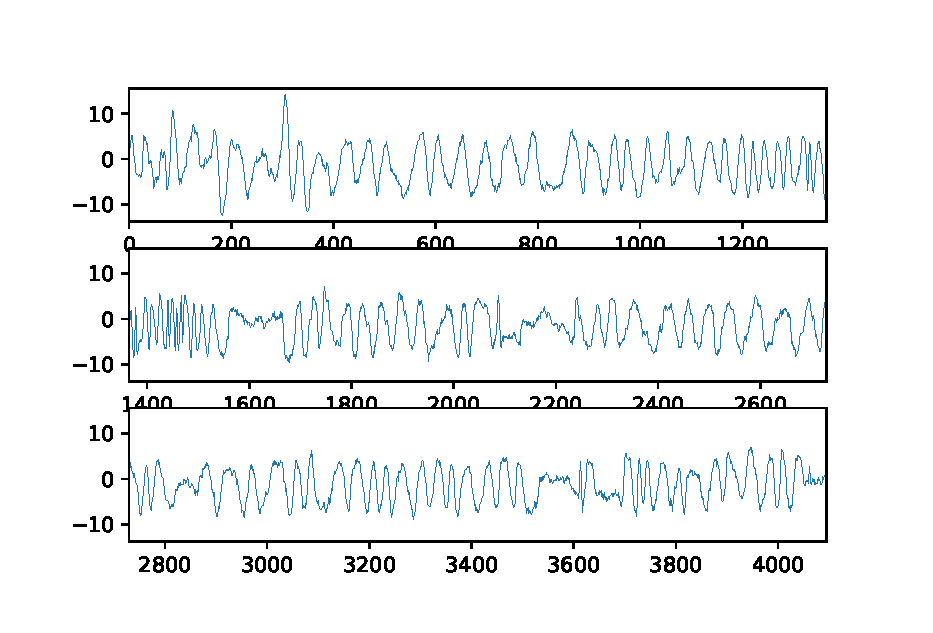
\includegraphics[width=\linewidth]{immagini/centro_di_massa-x.eps}
		\caption{Posizione y del centro di massa fotogramma per fotoframma}
		\label{fig:cmy}
	\end{figure}
\end{document}